\chapter{Introduction} \label{ch:introduction}
\newpage
%\section{Section}
%\subsection{SubSection}
%\subsubsection{SubSubSection}
%\paragraph{Paragraph}
%\subparagraph{SubParagraph}

\section{Perturbations to People}

Imagine you are standing on the corner of a busy Manhattan street. Every minute that passes shows the liveliness of a dynamic system, built up over many years. On an average block, there are approximately 28,154 people in the surrounding square kilometer, and a total of 1.7 million people on the island \citep{manhattan_population_density}. In contrast, a mere 300 years ago, the population was more disperse, and numbered in the thousands \citep{history_of_nyc}. Collections of thousands of people, initially spread out, came together to form a massive, dynamic ecosystem that represents an epicentre of modern human innovation and industry. Manhattan is not unique; cities across the world did not appear overnight, but were constructed hierarchically. It is in a similar fashion that modern astrophysics believes our Milky Way, and all massive galaxies formed with stars and gas as their building blocks.

We believe that the Universe began with a period of rapid inflation, and that in the process of this inflation, pockets of the Universe emerged more dense than other regions. This is revealed to us through observations of the cosmic microwave background (CMB). The CMB is a portrait of the Universe when it was last opaque; before electrons, neutrons, and protons combined to form the first atoms. It shows temperature fluctuations, like small population overdensities, that would eventually become cosmic cities.  While many physicists marvel at the physics that happens in these first moments of time, there is another story of how cosmic villages come together to form cities. This is the story of how tiny perturbations evolve to the structures astronomers see today.

When we look at the CMB, we are seeing the temperature distribution of matter through the radiation of baryonic matter, the matter that interacts with light. There is strong observational evidence to suggest that a large fraction of the matter present at this epoch is not interacting with light. This evidence is found in the power spectrum of the CMB, a function that describes the distribution of scales of the perturbations in the CMB \citep{transfer_fn}. 

This dark matter appears to be present in the current epoch. Evidence of dark matter in modern-day galaxy clusters was first observed by \citet{zwicky_1933}, who inferred that the mass of the Coma Cluster needed to be approximately ten times higher than observed to explain the motions of the constituent galaxies. A convincing case for dark matter in individual galaxies was presented by \citet{rubin_1980}, who show that the rotational speeds of stars in the disks of galaxies were too high to be explained by observed mass.

Based on enormous observational evidence, the dark matter component of the Universe appears to be substantial. If the results from the Planck satellite are taken as truth, then dark matter comprises around 84\% of all matter in the Universe \citep{planck_2018}. Dark matter influences the evolution of galaxies not only because it is not subject to radiation-based interactions, but also because it is most of what there is. Dark matter is the glue that holds galaxies together.  

Although dark matter makes up 84\% of the matter, matter only makes up 31.5\% of the present day Universe's total energy density. The remainder contains a modest contribution from radiation, but the bulk is comprised of unaccounted dark energy \citep{kolb_turner,dodelson, BT}. Dark energy, whatever it is, is responsible for the accelerating expansion of the Universe, something we first learned from observations of Type 1a supernova \citep{reiss_1998,perlmutter_1999}. Modern cosmology is a struggle between the competing forces of dark matter and dark energy, and both have implications for the local dynamics in the Universe.

To understand how dark matter is interacting with galaxies, we need to pin down its dynamics. This depends on what dark matter actually is. Some candidates, such as neutrinos, are relativistic particles that constitute hot dark matter. Warm and cold dark matter candidates become progressively non-relativistic, and there are many candidate particles for these models. An interesting and currently active proposal is that massive WIMPs, which were relativistic and coupled to baryons at early times, but cooled as the Universe expanded.

A model of the Universe one might consider is one comprised of cold dark matter and dark energy, described on large scales by a single parameter, $\Lambda$. This paradigm is called $\Lambda$CDM and is the prevailing model in the astronomy community. The model has been enormously successful in explaining observations, including the CMB power spectrum. While there remain open problems with $\Lambda$CDM, it appears to predict many properties on Galactic and extragalactic scales correctly \citep{kolb_turner,dodelson, BT}. Proposals to modify $\Lambda$CDM tend to present only slight variations on the model, such as allowing for self interacting dark matter (SIDM).
\begin{figure}
	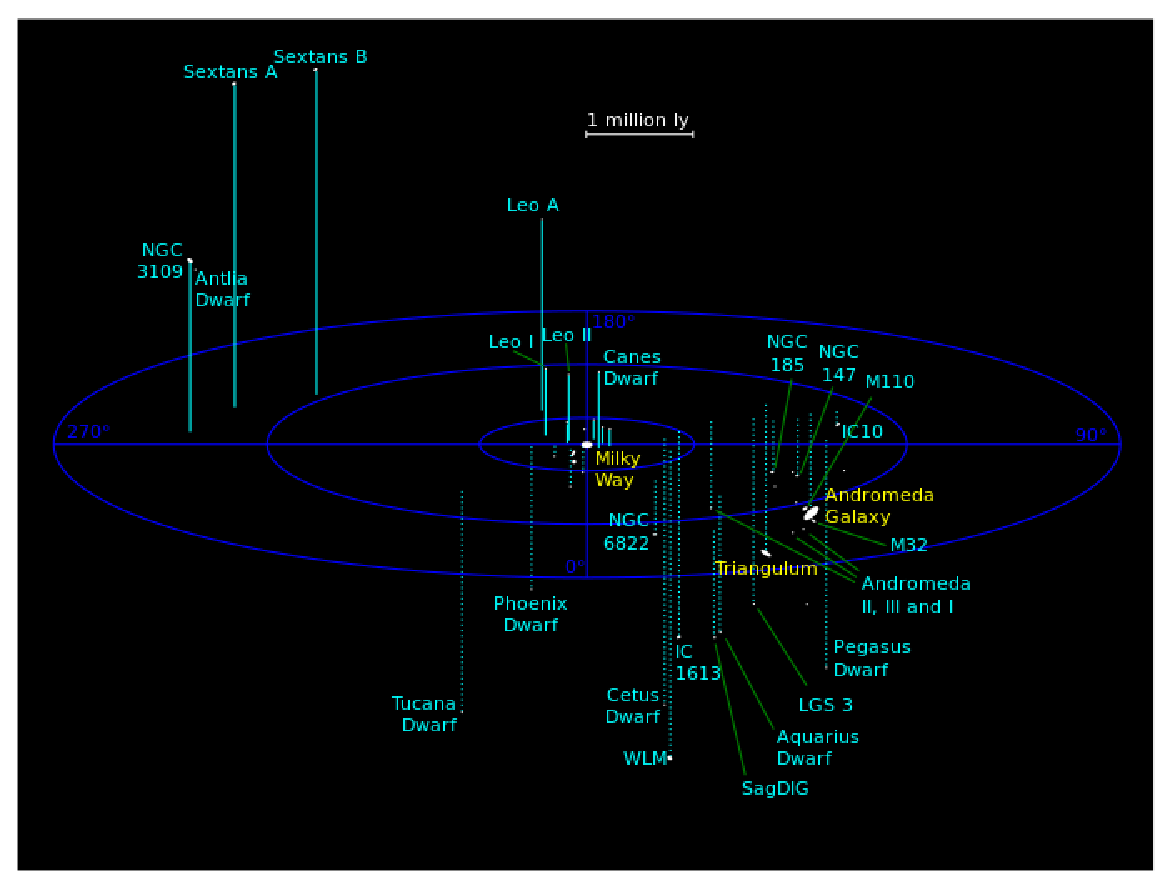
\includegraphics[width=\textwidth]{../figures/local_group}
	\caption{A map of the Local Group obtained per the license in \citet{local_group_map}.}\label{fig:local_group}
\end{figure}


%\subsection{The Story of the Milky Way}
Taking $\Lambda$CDM as the ground truth, we can begin to understand how galaxies evolved from tiny villages. Dark matter, which does not interact through any force but gravity, retains a perturbed structure after inflation. The density perturbations collapse, forming potential wells of dark matter \citep{taylor_2011}. The exact manner in which this happens is \textit{linear}, meaning that the amplitude of the perturbations increases proportionally with the expansion of the Universe, as measured by the scale factor. 

The baryons, interacting through baryon acoustic oscillations (BAO), are delayed in falling into the potential wells made by the dark matter. As the baryons fall into the centers of the potential wells over time, the cores of the dark matter distributions, comprised of spheroidal structures called halos, contract. After infall into a dark matter halo, the baryons cool to the point where stars are able to form. This is how the first galaxies formed. 

Over time, galaxies begin to shift away from the linear mapping between perturbation and galaxy. Their forces on each other start to matter locally, and galaxies begin to merge hierarchically. Collections of galaxies form, sometimes massive clusters of $10^{15}$ solar masses. Other times, groups with a couple massive galaxies become host to many smaller galaxies called subhalos. Other galaxies belong to no group or cluster, and exist in the expansive void between clusters. Dark energy continues to pull the Universe apart, while locally galaxies are kept together by dark matter. Merging of galaxies continues on local scales as larger galaxies become larger, bringing us to today.

We live in a spiral galaxy of approximately $10^{12}$ solar masses (dark matter + baryons), in a group with another galaxy, M31 (Andromeda), which has a roughly similar mass. Our Local Group (Fig. \ref{fig:local_group}), as it is called, is comprised of many smaller galaxies. In our Milky Way's halo, for instance, a merger is beginning between the Milky Way and the Large and Small Magellanic Clouds (LMC/SMC), shown in the third quadrant of the inner circle around the Milky Way in Fig. \ref{fig:local_group}. The SMC/LMC systems total approximately 10-20\% of the Milky Way's mass in total \citep{erkal_lmc}. Most of our subhalos are not nearly this massive, although they number in the hundreds. The picture painted of the Local Group is that of M31 and the Milky Way devouring smaller galaxies. Of course, this will have a substantial impact on the evolution of the stars in the Milky Way, and is the crux of this thesis. By studying the Milky Way's local environment, we can hope to understand the interactions dark matter has on baryons, and perhaps infer something about how dark matter is distributed in our Galaxy.

%...the current de facto standard being the Unified Modeling Language
%(UML)~\cite{BRJ99}...

%\section{Problem}

%\section{Objective}

%\notesbox{Note:  These are the section headings that I decided to use.  Check out several
%recent theses to decide how you want to lay out your introduction (and conclusion) chapters.}


%\subsection{Hypothesis}

\section{Understanding $\Lambda$CDM with Galaxy Simulations}

Many of the hardest questions in Galactic astrophysics stem from the fact that dark matter is not directly observable. As an example, what is the underlying smooth distribution of dark mass? How many dark matter subhalos should the Milky Way have? What is the effect on large scales if we choose something other than $\Lambda$CDM? While these questions are not easily answerable by direct observation, we can complement indirect observations with a solid theoretical understanding to reach confident answers.

Simulations link theory and observations, allowing the theory to be tested. When a simulation is performed, theoretical input is considered. This includes a model of cosmology, or a model of the galaxy, the nature of dark matter, etc. All of this knowledge is reduced to a fluid system which may be solved through numerical techniques on a computer.  The output of the simulation can then be compared to observations to test the underlying theory's validity.

Over the last four decades, many tools have been developed to study the structure of the present day Universe. These tools have become increasingly sophisticated as computation power and algorithms research advance. One tool is an \textit{ab initio} cosmological simulation, which simulates the entire formation history of the Universe from some informed initial density field.  This initial density field is derived from the primordial power spectrum and early-Universe baryon physics, and a sample can be drawn and evolved with periodic boundary conditions \citep{music}. If done correctly, this creates a representative sample of many structures in a $\Lambda$CDM Universe. Halos evolving in these simulations feel the full effect of the completely simulated cosmological environment. Such simulations stand in contrast to isolated galaxy simulations, which seek to explain the detailed dynamics arising from generic effects in individual galaxies. These simulations start with a prescription for what an equilibrium galaxy looks like, and study the evolution of galaxies initialized from these prescriptions. While missing some critical cosmological physics, these simulations may be run at very high resolution.


This thesis studies dynamics on a Galactic scale. Through simulations of galaxies, we can understand how dark matter influences their evolution. $\Lambda$CDM has been tested in this way for decades, and we detail some global results in what follows. In particular, we focus on where simulations of galaxies have shown discrepancies in cosmological theory.

We broadly commented on the hierarchical formation of galaxies. Over time, galaxies that merge with other galaxies should become well-mixed in the host halo. That is, there should be an underlying smooth distribution of mass in which all of the subhalos reside. A key prediction of $\Lambda$CDM is that this smooth distribution should have a universal density profile in the limit that dark matter dominates the Universe \citep{nfw}. Furthermore, the dark matter should have a density distribution somewhat resembling a squashed football, a spheroid flattened on two axes, in general. There are, in fact, the special cases of being either perfectly spherical, prolate, or oblate. Whether or not this picture holds observationally in real galaxies is an open problem. The density profile proposed by \citet{nfw} is cuspy at the center, whereas some observations are more consistent with a flatter central density \citep{de_blok_core_cusp}. Astronomers have dubbed this the Core-Cusp Problem. 

Besides the Core-Cusp Problem in the inner parts of dark matter haloes, one thing that is clear is that $\Lambda$CDM halos should have many subhalos. As the general theory for the formation of galaxies goes, these subhalos were at one point independent perturbations that have since merged into the Milky Way's halo, and should have their own stellar and gas content. This means that we expect many massive subhalos to be directly observable. Another triumph of simulations is putting an actual number on how many subhalos we expect from $\Lambda$CDM. Surprisingly, far fewer subhalos are actually observed \citep{mooresubhalos, Klypin1999, springel2008}. This discrepancy has since been dubbed the Missing Satellite Problem, and is an open problem for $\Lambda$CDM and astronomy.


The Core-Cusp Problem and Missing Satellite Problem have received a lot of attention in the literature because of the potential problems they pose for theoretical cosmology. It is clear that to accurately recover the global properties of substructure on large scales, dark matter must be cold. Warm and hot dark matter models\footnote{Hot dark matter is comprised of matter moving at or near the speed of light (e.g. neutrinos), and warm dark matter is somewhere in between cold and hot dark matter.} simply do not yield substructure populations consistent with observations \citep[for example]{alternate_dm}. SIDM and fuzzy models, where the dark matter can interact on small scales, have been proposed as slight modifications to the $\Lambda$CDM paradigm, with some success \citep[for example]{hui_2017}. 

Despite the presence of alternate theories of cosmology, a large concerted effort has been made to understand discrepancies as a byproduct of baryonic physics.  Adequate explanation of halo and substructure response to stellar and gas content would mean that alternate cosmologies are not necessary to explain the Core-Cusp Problem and Missing Satellite Problem. Initially, \textit{ab initio} simulations included only dark matter, but have evolved over the last three decades to consider very sophisticated subgrid models of gas physics and star formation \citep{LucySPH,CenOstriker92,KatzSPH96,SpringelMultiphase03,Stinson2006}.  These simulations can be used to realize the galaxy formation predicted by current theories. State of the art unigrid (single resolution) cosmological simulations struggle to compete with the resolution attainable by isolated galaxy simulations \citep{Illustris,Eagle}, but they can still be used to make broad statements about consistency with $\Lambda$CDM. Broadly speaking, it is not clear at this stage whether or not apparent issues with $\Lambda$CDM can be resolved through these models, but they present a promising approach as computing power is sure to increase.

%Because of resolution factors, the goal of many of cosmology studies has shifted from studying galaxy dynamics to reproducing population statistics such as scaling relations.  As a consequence, problems which are at the interface of the complex cosmological environment and individual galaxy dynamics are still open.

All of the preceding is to say that simulations are an enormously valuable tool in understanding the broad predictions of cosmology on a Galactic scale. We have used them to uncover apparent inconsistencies in $\Lambda$CDM, and have a promising means within the paradigm to move forward in resolving these inconsistencies. All of the preceding discussion has focused on the complexity of the halo environment. Ultimately, we are looking for simulations to make observable predictions, and specifically signatures outside the Galactic halo that theory is correct.

\section{Dynamical Processes in a Chaotic Milky Way}

Since dark matter is not directly probable, we must use indirect methods to infer information about the halo. For this, we need to know something about the distribution of mass in the Galaxy.

\subsection{Distribution of Mass in the Milky Way}

In addition to the dark matter halo, our Galaxy is composed of baryons in the form of a central spheroidal bulge, a thin gas disc, a thin stellar disc, and a more diffuse thick stellar disc. The thin stellar disc is where the majority of our work is focused. We see a wide variety of structure in the stellar discs of other galaxies, as well as our own Milky Way. For example, the center of our galaxy is believed to contain a stellar bar, a bar-like component of the thin disc \citep{BT}. There are also non-planar features in stellar discs, such as warps \citep{BT}. How these features come into being is a main focus of this thesis.\footnote{For an in-depth discussion of the features arising in stellar discs, \citet{Sellwood2013} presents a fantastic review.}

There is also a stellar component of the halo, which contains remnants of old mergers and star clusters known as globular clusters. This section is organized by talking about tidal disruption of subhalos in the Galactic halo, the dynamics of the central part of the Galaxy, and vertical structure in the Galactic disc. How the cosmological environment effects these observables is the bulk of this thesis, and we motivate here why these aspects are the subject of focus.

\subsection{Stellar Streams from Mergers}

In the hierarchical formation of galaxies, smaller galaxies merge with larger galaxies and become a part of the larger galaxy's halo. As subhalos become more a part of the host system, they experience tidal forces that stretch and squeeze their mass content. Dark matter and stellar material is stripped from these merging galaxies over time to form streams of tidal debris. In the long run, this debris will equlibrate with the stellar halo. It should be noted that the same effects apply to globular clusters too.

Baryonic debris left behind can detected. The first stream for which this accomplished was the debris of the Sagittarius Dwarf Spheroidal galaxy (Sgr dSph), a dSph galaxy discovered by \citet{ibata_discovery}. The corresponding stream was later detected by \citet{newberg_2002} and \citet{majewski_2003}. 

These discoveries of debris associated with a merging dwarf galaxy kickstarted an onslaught of literature based on the detection of streams, and their potential uses in probing the Galactic potential. The general idea is that so long as streams approximately trace orbits in the halo, the correct Milky Way potential, dark matter and all, is the unique potential that reproduces these orbits. 

More streams have been discovered since then, and a few notable ones are the Orphan Stream \citep{grillmair_2006,belokurov_2007,newberg_2010}, remarkable for its apparent lack of progenitor, TriAnd, A13, and the Monoceros Ring. This is by no means a complete accounting of known stellar streams. Something on the order of nearly a hundred known to exist in the Milky Way alone \citep{sanders_binney_2013_a, ibata_2019}. While streams alone have been useful in getting some broad constraints on the Galactic potential and geometry of the halo, complications arise from the fact that streams do not follow orbits exactly \citep{sanders_binney_2013_a} and the fact that the Milky Way potential is predicted from theory to be time dependent.

The orbits of streams are not the only way to learn about the Milky Way's dark matter halo. It is worth mentioning that there is the possibility of using the fine structure of stellar streams to learn more about the subhalo population in the halo.  Gaps form when subhalos pass through tidal streams, and this is one direction that is being explored for leveraging stellar stream data (e.g. \citet{erkal_2016_stream_gaps}).

%With the Sagittarius stream specifically, there 
\subsection{Response of the Galactic Disc to the Cosmological Environment}


We might also attempt to infer properties of the subhalo population through their effect on the Galactic disc.  It is believed that the affect of the Milky Way's substructure population can be observed as wave-like behaviour in the thin disc's vertical structure \citep{widrow_2012_sdss,carlin_2013_lamost, williams_2013_rave,xu_2015, carrillo_2018_rave}.  These waves can manifest as small corrugations in the Galactic disc, as global bending and breathing motions, or even as large warps in the Milky Way's gas  \citep{gasWarp} and stellar discs. It is worth noting that these observations are being confirmed in DR2 of the Gaia mission \citep[for example]{gaia_collab,bennet_2019_gaia}.

The Milky Way's massive subhalos are most likely inducing non-planar density patterns in the disc, and we would like to understand the nature of these patterns through simulation. Unfortunately, we need the high resolution of isolated galaxy simulations to study these effects, and the realism of an \textit{ab initio} Galactic halo.  This has motivated a long history of attempts to bridge the gap between {\it ab initio} cosmological simulations and those of isolated galaxies.  A particularly simple class of simulations involves the interaction of a disc
with a single satellite galaxy or dark matter subhalo.  For example \citet{kazantzidis2008} perform simulations in which a thin Milky Way-like disc is subjected to a series of encounters with a satellite.  The masses and orbital parameters of the satellites are motivated by substructure found in a halo appropriate to a Milky Way-like galaxy from a cosmological simulation.  Their simulation demonstrated that satellite encounters lead to general disc heating as well as distinctive disc features such as bars, spiral structure, flares, and rings.  \citet{purcell2011} model the response of the Milky Way to the gravitational effects of
the Sgr dSph by simulating disc-dwarf encounter for different choices of the Sgr progenitor's mass.  Their conclusion is that Sgr may have triggered the development the spiral structure seen today in the Milky Way.  This approach has gained considerable traction in the last couple years, with authors using single-satellite encounters to explain the existence of low-latitude streams and other vertical structure in the Milky Way's disc \citep[for example]{widrow_2014, dlv_2015, donghia_2016, laporte_2016, laporte_2018}. One particularly interesting feature arising from these works is that stars may occasionally be kicked out of the galactic disc to form kicked-up disc populations \citep{johnston_kud_review, laporte_2019_feathers}. Such populations may explain low-latitude Milky Way structures, and possibly kinematic data of M31 \citep{dorman_2013_m31}.

% Say something about KUD since you will focus on it. One interesting feature... Which might explain MW M31

Of course, the disc of the Milky Way lives within a population of satellite galaxies and, quite possibly, pure dark matter subhalos, and single-satellite encounters do not describe the complexity of the cosmological environment \citep{Klypin1999,mooresubhalos,springel2008}.  With this in mind \citet{Font2001} simulated the evolution of an isolated disc-bulge-halo model where the halo was populated by several hundred subhalos.  They concluded that that substructure played only a minor role in heating the disc, a result that would seem in conflict with those of the \citet{kazantzidis2008} that would come later.  Numerical simulations by \citet{gauthier2006, dubinski2008} sheds some light on this discrepancy.  In these simulations, 10\% of the the halo mass in an isolated disc-bulge-halo system is replaced by subhalos with a mass distribution motivated by the cosmological studies of \citet{gao2004}.  In the \citet{gauthier2006} simulation, little disc heating occurs during the first 5 Gyr, at which point satellite interactions provoke the formation of a strong bar, which in turn leads to significant heating.  Not surprisingly, when the experiment is repeated with different initial conditions for the satellites the timing of bar formation can vary.  These experiments also suggest that a large fraction of the mass initially in subhalos is tidally stripped leaving behind a complex system of tidal debris.

The aforementioned simulations, although more realistic than single-satellite encounters, have three main problems.  First, they don't allow for halo triaxiality.  Secondly, the disc is initialized at its present-day mass whereas real stellar discs form over several Gyr.  Finally, the subhalo populations are inserted into the halo by hand.  While the mass and spatial distributions of the subhalos are motivated by cosmological simulations, they may not capture important properties of realistic halos. This has historically been solved by modifying a traditional \textit{ab initio} simulation. The zoom-in technique (a Monte Carlo adaptive mesh) is used to study the evolution of a disc in a single halo at high resolution.  This is accomplished by resampling the initial conditions at a sequence of higher resolutions after identifying an area of interest. With sufficiently realistic feedback, impressively realistic results can be obtained. For instance, \citet{gomez_2017} presented a study of vertical structure in such simulations. In these simulations, the authors were able to look at several Milky Way-like galaxies in a variety of environments at resolutions that rival isolated galaxy simulations. These realistic studies have opened the door to a wide variety of questions pertaining to the Milky Way's interaction with the cosmological environment.

\section{Disc Insertion Techniques for Cosmology}

While highly realistic, the \textit{ab initio} zoom-in approach still suffers from the inability to fine-tune galaxy dynamics in the same halo to perform a truly systematic study. In an effort to address these particular shortcomings, several groups have attempted to grow a stellar disc in a cosmological halo.  

% Should add a footnote about redshift

The general idea for growing a disc is to divide a zoom-in simulation into three phases.  During the first, a cosmological simulation of a region of interest is run, and a halo is identified for study.  A rigid disc potential is then slowly grown in this halo, allowing the halo particles to respond adiabatically to its time-varying potential.  Finally, the rigid disc is replaced by live particles and the final phase of the simulation proceeds with live disc and halo particles.  \citet{debuhr_2012} use this scheme to introduce stellar discs into dark matter halos from the Aquarius Project \citep{springel2008}.  They add a rigid disc potential at redshift $z=1.3$ with a mass parameter for the disc that grows linearly with the scale factor until $z=1$ when it reaches its final value.  The disc potential is initially centered on the potential minimum of the halo and oriented so that its symmetry axis points along either the minor or major axis of the halo.  During the rigid disc phase, the centre of the potential moves due to its interaction with the halo (Newton's 3rd law) so that linear momentum is conserved.  However, the orientation of the disc is held fixed and therefore angular momentum isn't.  To initialize the live disc, \citet{debuhr_2012} approximate the halo potential as a flattened logarithmic potential and then determine the disc distribution function by solving the Jeans equations in axisymmetry. 

A number of refinements to this scheme were introduced by \citet{ys_2015}.  In particular, they use the GALIC code to initialize the live disc \citet{YurinSpringelGalic}.  This code aims to find a stationary solution to the collisionless Boltzmann equation by adjusting the initial particle velocities so as to minimize a certain merit function.  In \citet{ys_2015} the initial disc distribution function was assumed to depend on two integrals of motion, the energy $E$ and angular momentum $L_z$.  Consistency then required that they use an axisymmetrized approximation to the halo potential.

\citet{bauer2018a} improved on the scheme even further by increasing the realism of the growth phase by modelling the disc as a rigid body. The results they found were qualitatively similar to \citet{debuhr_2012} and \citet{ys_2015}  in terms of disc dynamics. The live phase was also improved by using the \textsc{GalactICS} code which actually samples a three-integral DF. This thesis is largely constructed based on this tool.


\section{Organization and Findings of this Thesis}

By applying our disc insertion tool, we address three key scientific questions. The first is how growing a disc in a cosmological halo affects the halo itself. Here, we attempt to understand how the way we grow the disc affects halo properties. The second is how bars form in cosmological environments. Previous studies using disc insertion techniques found that stellar discs all form very large bars. Large central bulges were found in \citet{ys_2015} to have an ameliorating affect. We explore the reasons why their disc-halo systems formed large bars, and show how we can form bars similar to the Milky Way's without including a large central bulge. The last topic we consider is how vertical structure is excited in the Milky Way. We explore the combined effect of mechanisms in the cosmological environment, and comment on how significant factors like substructure, tides, and bar buckling are for the Milky Way.

The thesis is organized in the following manner. In Chapter~\ref{ch:background}, we reduce the necessary theoretical background to understand this work to a succinct summary. Following this, in Chapter~\ref{ch:paper_i}, we explore the first peer-reviewed paper on which this thesis is based. It outlines the disc insertion scheme and comments on how the dynamic nature of the Milky Way's stellar disc should affect its inner halo. Chapter~\ref{ch:paper_ii} presents the second published paper which focuses on the question of how stable disks are against forming bars in a cosmological setting. A final paper is presented in Chapter~\ref{ch:paper_iii}, where we look at how disks form vertical structure in a cosmological setting. We conclude with summaries and ideas for future work in Chapter~\ref{ch:conclusion}.

\bibliographystyle{apalike}
\bibliography{bibliography_introduction}